% !TEX root = main.tex

\section{Sensitivity studies}


\subsection{PDF}

First, I define the purely hadronic amplitudes for a given phasespace point $x$.
The weak phase dependence is written latter explicitly in the pdf.

%\begin{align}
%	A(B_s^0 \to D_s^{-} K^{+} \pi\pi) &\equiv A(x) = \sum_i a_i \, A_i(x)   \\
%	A(\bar B_s^0 \to D_s^{-} K^{+} \pi\pi) &\equiv \bar A(x) = \sum_i \bar a_i \,\bar A_i(x)   \\
%	A(\bar B_s^0 \to D_s^{+} K^{-} \pi\pi) &= A(x)  \, \, \text{(Assuming no direct CPV)} \\
%	A(B_s^0 \to D_s^{+} K^{-} \pi\pi) &= \bar A(x)  \, \, \text{(Assuming no direct CPV)} 
%\end{align}

\begin{align}
	A(B_s^0 \to D_s^{-} K^{+} \pi\pi) &\equiv A(x) = \sum_i a_i \, A_i(x)   \\
	A(B_s^0 \to D_s^{+} K^{-} \pi\pi) &\equiv \bar A(\bar x) = \sum_i \bar a_i \,\bar A_i(\bar x)    \\
	A(\bar B_s^0 \to D_s^{-} K^{+} \pi\pi) &= \bar A(x)  \, \, \text{(Assuming no direct CPV)} \\
	A(\bar B_s^0 \to D_s^{+} K^{-} \pi\pi) &= A(\bar x)  \, \, \text{(Assuming no direct CPV)} 
\end{align}

The full time-dependent amplitude pdf is given by:
\begin{equation}
\begin{split}
\label{eq:PDF_full}
	P(x,t,q_t,q_f) &\propto  [
	 \left( \vert A(x) \vert^2 + \vert \bar A(x) \vert^2 \right) \, \text{cosh} \left( \frac{\Delta \Gamma \, t}{2}\right) \\
	 & + q_t q_f \left( \vert A(x) \vert^2 - \vert \bar A(x) \vert^2 \right) \, \text{cos} \left( m_s \, t \right)  \\
	 & -2 \text{Re}\left( A(x)^{*}  \bar A(x) \, e^{-i q_f (\gamma - 2\beta_s)}  \right) \, \text{sinh} \left( \frac{\Delta \Gamma \, t}{2}\right)  \\
	 & -2 q_t q_f \text{Im}\left( A(x)^{*}  \bar A(x) \, e^{-i q_f (\gamma - 2\beta_s)}  \right)\, \text{sin} \left( m_s \, t \right)  ]  e^{- \Gamma t}
\end{split}
\end{equation}
where $q_t = +1$ $(-1) $for a $B_s^{0}$ ($\bar B_s^{0}$) tag and 
$q_f$ = +1 $ $(-1) for $D_s^{-} K^{+} \pi\pi$ ($D_s^{+} K^{-} \pi\pi$) final states. \\

Integrating over the phasespace, we get
\begin{equation}
\begin{split}
\label{eq:PDF_intX}
	\int P(x,t,q_t,q_f) \text d x &\propto   [
	\, \text{cosh} \left( \frac{\Delta \Gamma \, t}{2}\right) \\
	 & + q_t q_f \left( \frac{1-r^2}{1+r^2} \right) \, \text{cos} \left( m_s \, t \right)  \\
	 & -2 \left( \frac{\kappa \, r \, \text{cos}(\delta - q_f(\gamma - 2 \beta_s))}{1+r^2}  \right) \, \text{sinh} \left( \frac{\Delta \Gamma \, t}{2}\right)  \\
	 & -2 q_t q_f \left( \frac{\kappa \, r \, \text{sin}(\delta - q_f(\gamma - 2 \beta_s))}{1+r^2}   \right)\, \text{sin} \left( m_s \, t \right)  ]  e^{- \Gamma t} \\
	 &=   [
	\, \text{cosh} \left( \frac{\Delta \Gamma \, t}{2}\right) 
	  + q_t q_f \, C \, \text{cos} \left( m_s \, t \right)  
	  - \textcolor{red}{\kappa} \, D_{q_f} \, \text{sinh} \left( \frac{\Delta \Gamma \, t}{2}\right)  
	  - q_t \, \textcolor{red}{\kappa} \, S_{q_f}\, \text{sin} \left( m_s \, t \right)  ]  e^{- \Gamma t}
\end{split}
\end{equation}
where the $C,D_{q_f},S_{q_f}$ are defined exactly as for $D_s K$.
The coherence factor is defined as :
\begin{align}
\label{eq:coherenceFactor}
	\kappa \, e^{i\delta} &\equiv \, \frac{\int A(x)^{*}  \bar A(x)  \text d x}{\sqrt{\int \vert A(x) \vert^2\text d x} \sqrt{\int \vert \bar A(x) \vert^2\text d x}  } \\
	r &\equiv \, \frac{\sqrt{\int \vert \bar A(x) \vert^2\text d x }}{\sqrt{\int \vert A(x) \vert^2\text d x}} 
\end{align}
and appears in front of the $D_{q_f},S_{q_f}$  terms.
This means one additional fit parameter for the lifetime fit.
In the limit of only one contributing resonance $\kappa \to 1$. \\


\subsection{Estimation of coherence factor}

To estimate the coherence factor we could generate many toys with random $a_i$ and $\bar a_i$ values (see https://twiki.cern.ch/twiki/pub/LHCbPhysics/Bu2DKstar/LHCb-ANA-2017-005\_v1.pdf) using the set of amplitudes show in our last talk. However with so many interfering amplitudes, I would be surprised if you couldn't generate every possible value for $\kappa$. In any case, this would give us a  range where to expect possible values for $\kappa$. Worst case would be $0 \leq \kappa \leq 1$. \\

Assumptions:
	\begin{itemize}
		\item   $A(x) = \sum_i a_i \, A_i(x)$   \\
		 $\bar A(x) = \sum_i \bar a_i \, \bar A_i(x)$
		\item Use amplitudes from flavor-averaged, time-integrated fit
		 \item Draw random $a_i$ and $\bar a_i $ values
		 \item Constraints: \\
		 $\int ( \vert a_i  A_i(x) \vert^2 + \vert \bar a_i  \bar A_i(x) \vert^2 ) \, \text{d}x / N = F^{eff}_i $ \\
		 $r \approx 0.4 $ (ration of CKM elements)
	\end{itemize}
	
\begin{figure}[hp]
	\centering
		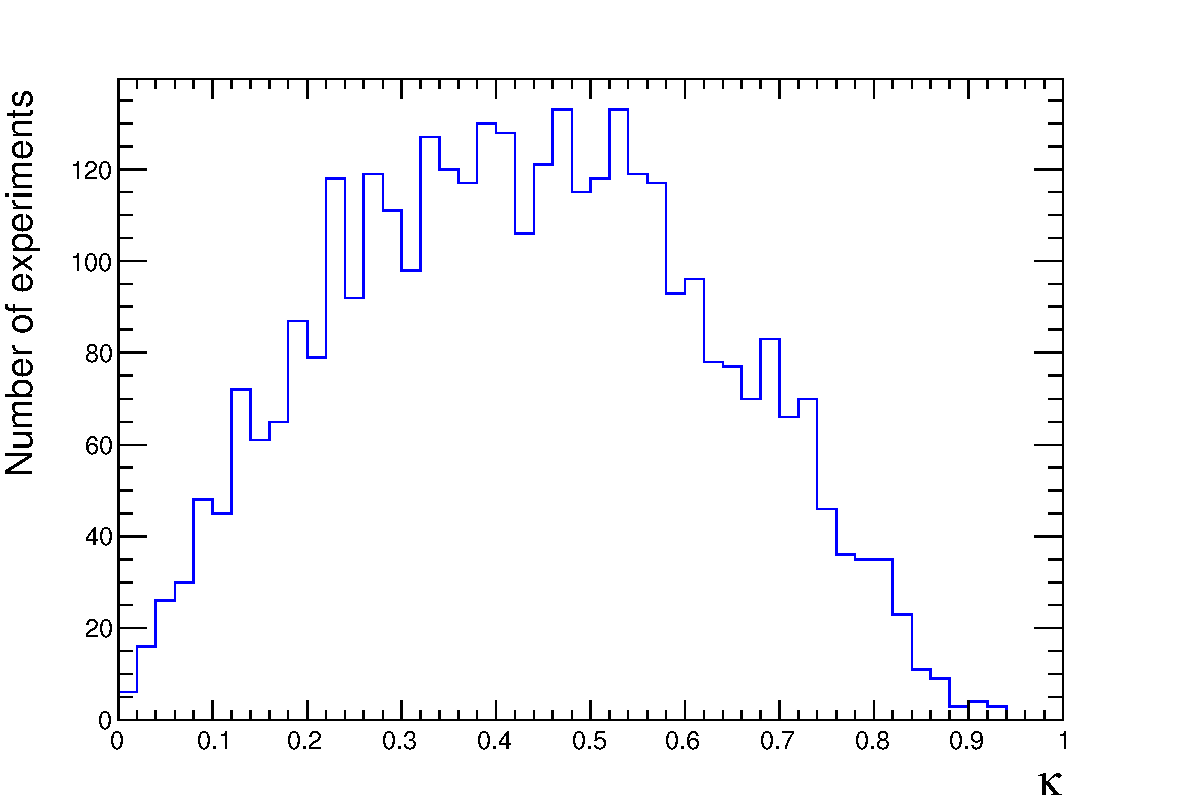
\includegraphics[width=0.35\textwidth, height = 3.cm]{figs/plots/k-eps-converted-to.pdf} 
		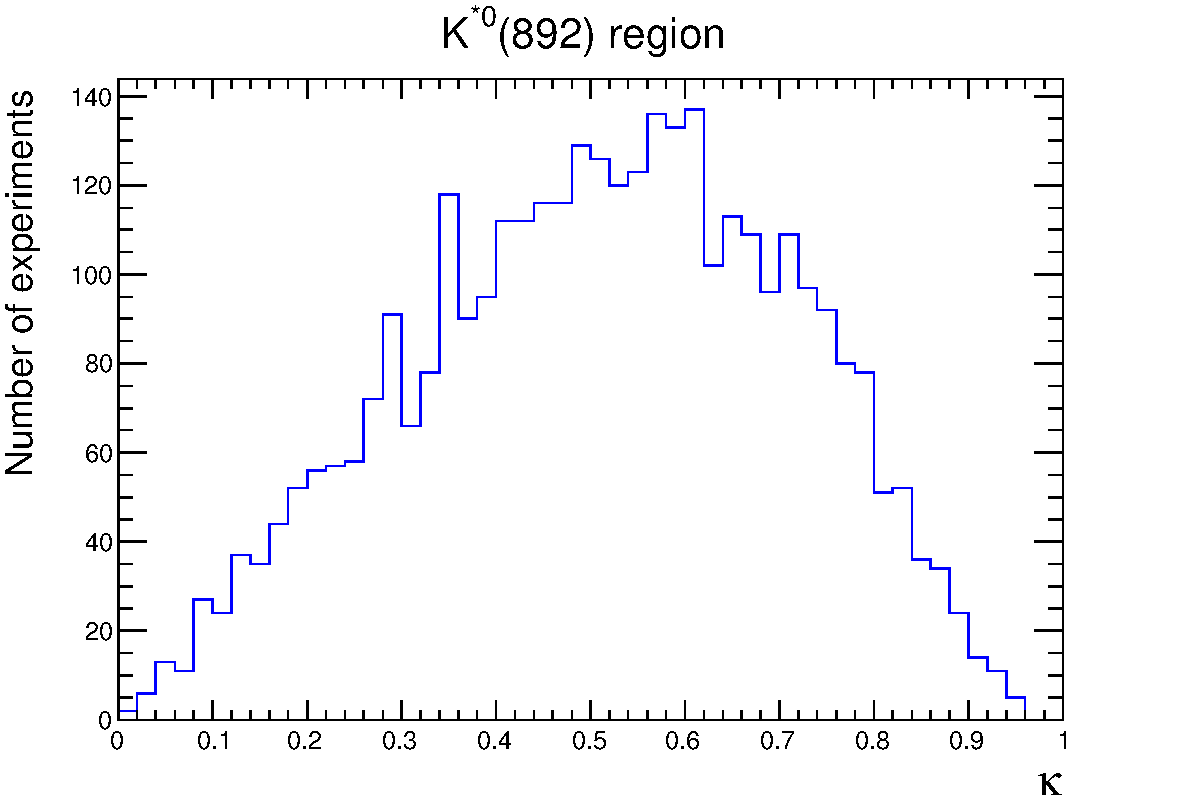
\includegraphics[width=0.35\textwidth, height = 3.cm]{figs/plots/k_Ks-eps-converted-to.pdf} 
		
		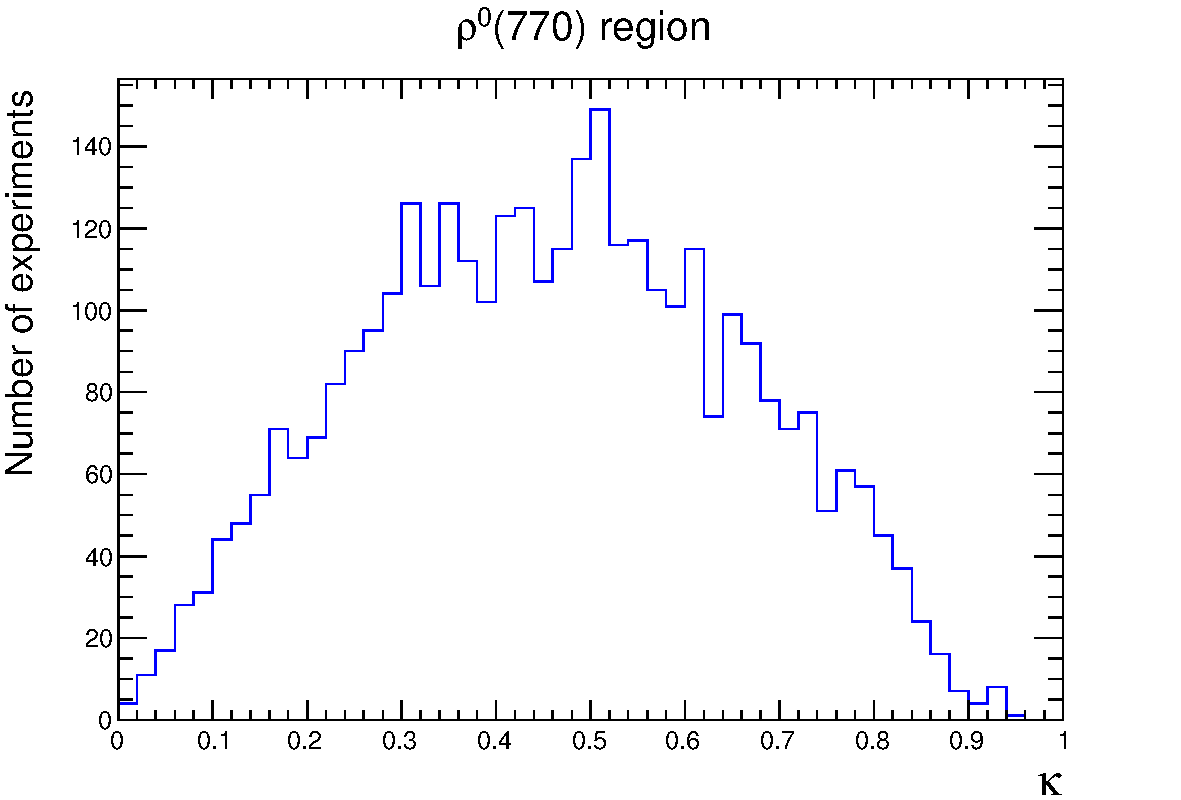
\includegraphics[width=0.35\textwidth, height = 3.cm]{figs/plots/k_rho-eps-converted-to.pdf} 
		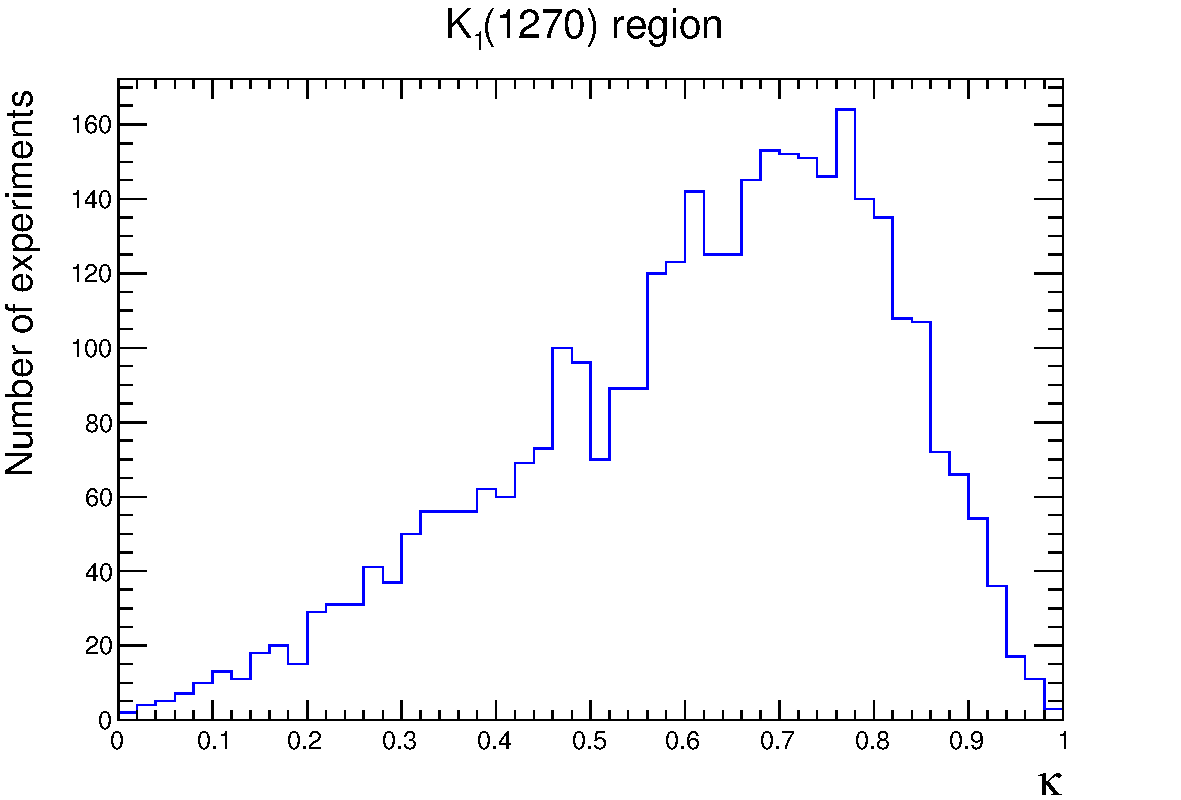
\includegraphics[width=0.35\textwidth, height = 3.cm]{figs/plots/k_K1-eps-converted-to.pdf} 	
		\caption{}	
\end{figure}		

	\begin{table}[h]
			\caption{}	
  \footnotesize
  \centering
  \begin{tabular}
    {l c c }
    \hline \hline
    Region &  $<\kappa> (\%)$   &  Cut eff. $(\%)$ \\   \hline
    Full & 43 &  100 \\
    $K^*(892)$ & 51    &  43  \\
    $\rho^0(770)$ & 46  & 47   \\
    $K_1(1270)$ & 61   & 23  \\
    \hline \hline
  \end{tabular}
  \label{tab:sideband}
\end{table}


%The next option would be to fit the flavor tagged Dalitz plot which would allow us to really predict $\kappa$ (together with $r$ and $\delta$ actually). 
%Integrating the full pdf over  time, we get
%\begin{align*}
%	\int P(x,t,q_t,q_f) \text d t &\propto   
%	 \left( \vert A(x) \vert^2 + \vert \bar A(x) \vert^2 \right) \, \frac{4\Gamma}{4\Gamma^2-\Delta \Gamma^2} \\
%	 & + q_t q_f \left( \vert A(x) \vert^2 - \vert \bar A(x) \vert^2 \right) \, \frac{\Gamma}{\Gamma^2+m_s^2} \\
%	 & -2 \text{Re}\left( A(x)^{*}  \bar A(x) \, e^{-i q_f (\gamma - 2\beta_s)}  \right) \,\frac{2\Delta\Gamma}{4\Gamma^2-\Delta \Gamma^2} \\
%	 & -2 q_t q_f \text{Im}\left( A(x)^{*}  \bar A(x) \, e^{-i q_f (\gamma - 2\beta_s)}  \right)\, \frac{m_s}{\Gamma^2+m_s^2} 
%\end{align*}
%
%I think that is a very interesting result since it shows that we could in principle also measure $\gamma$ with a time-independent 
%amplitude fit. But no idea how sensitive this would be. Probably not so much since the prefactors of the third and forth term are at least one order of 
%magnitude smaller than the first term.
%Unfortunately, the sensitivity to the coherence factor also comes mainly from the third and forth term. \\
%If we just want to estimate $\kappa$ from this fit and then use it for the lifetime fit, the potential $\gamma$ sensitivity of the Dalitz fit is another problem. 
%We could fix $\gamma$ to the world average for the dalitz fit but this might introduce some bias.
%Better would be to average over the final state flavor in which case the sensitivity to gamma would be lost. \\
%
%In summary, I think it is very hard to disentangle $A(x)$ and $\bar A(x)$ from a time integrated fit since the oscillation frequency is so large.
%We might be able to get some estimate but in the end, the lifetime fit has to determine the precise value.
%A full time dependent amplitude fit would of course be the most sensitive approach (but model-dependent).

\clearpage
\subsection{Results}

Assumptions:
	\begin{itemize}	
		\item Use amplitudes from flavor-averaged, time-integrated fit
		\item $r = 0.4$ (ratio of CKM elements) 
		\item PDG values for: $\tau,\Delta m_s, \Delta \Gamma, \beta_s$
		\item $\epsilon(x,t) = const.$, perfect resolution  
		\item $\epsilon_{Tag} = 0.66, <\omega> = 0.4 $   
		\item $N_{signal} = 3000$ (Run1+15/16 data)		 
	\end{itemize}
	
	
		\begin{figure}[hp]
	\centering
		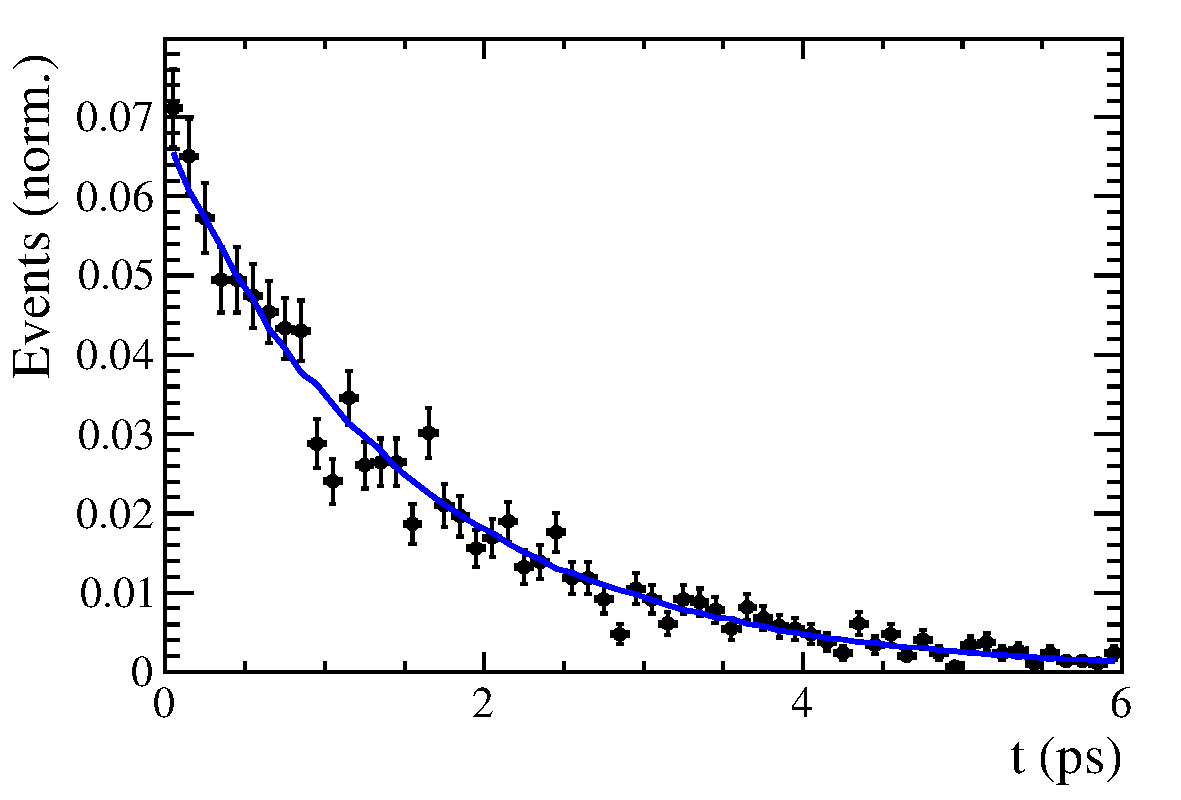
\includegraphics[width=0.45\textwidth, height = !]{figs/plots_toy/h_t-eps-converted-to.pdf} 
		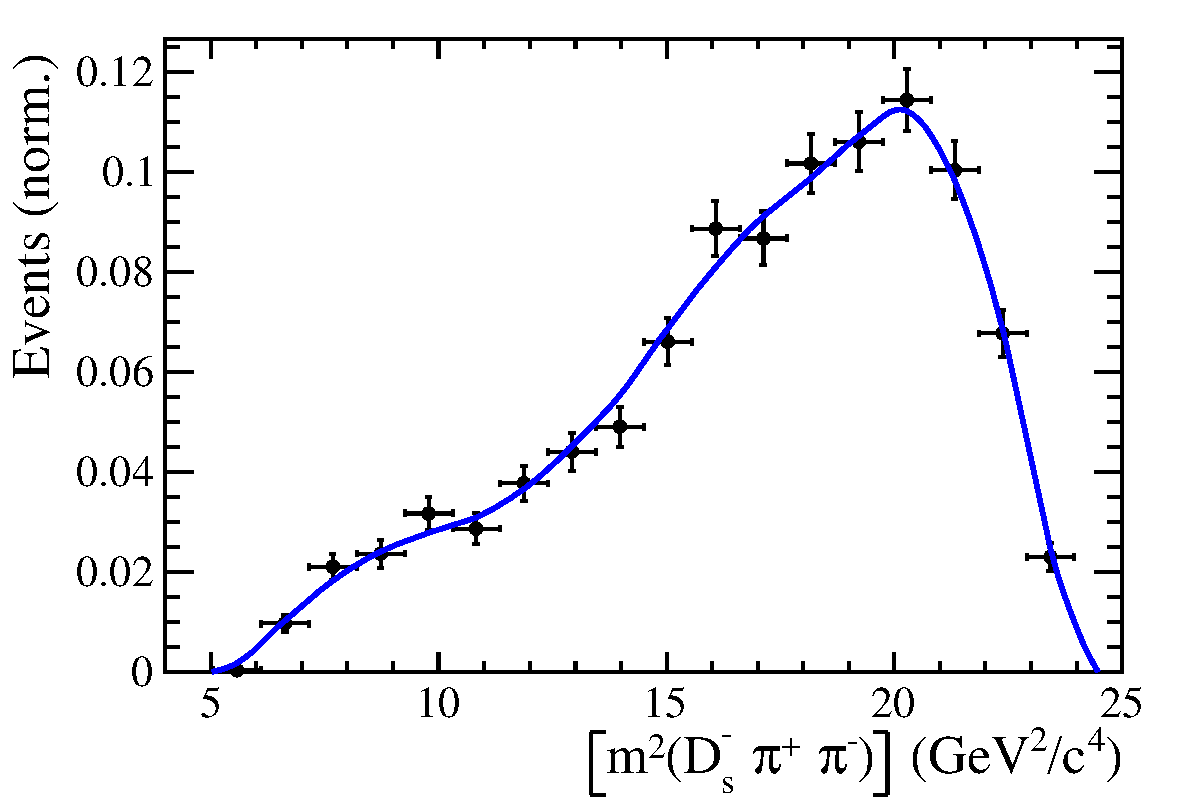
\includegraphics[width=0.45\textwidth, height = !]{figs/plots_toy/s_Dspipi-eps-converted-to.pdf} 
		
		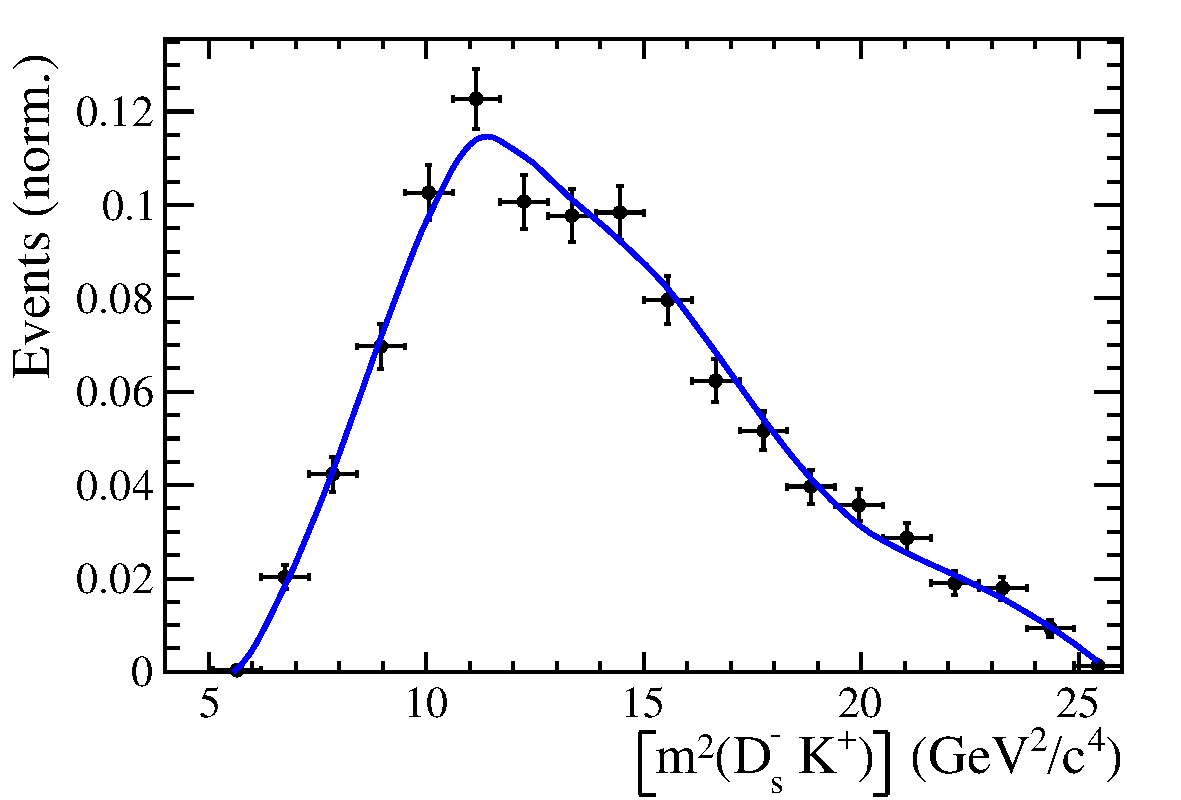
\includegraphics[width=0.45\textwidth, height = !]{figs/plots_toy/s_DsK-eps-converted-to.pdf} 
		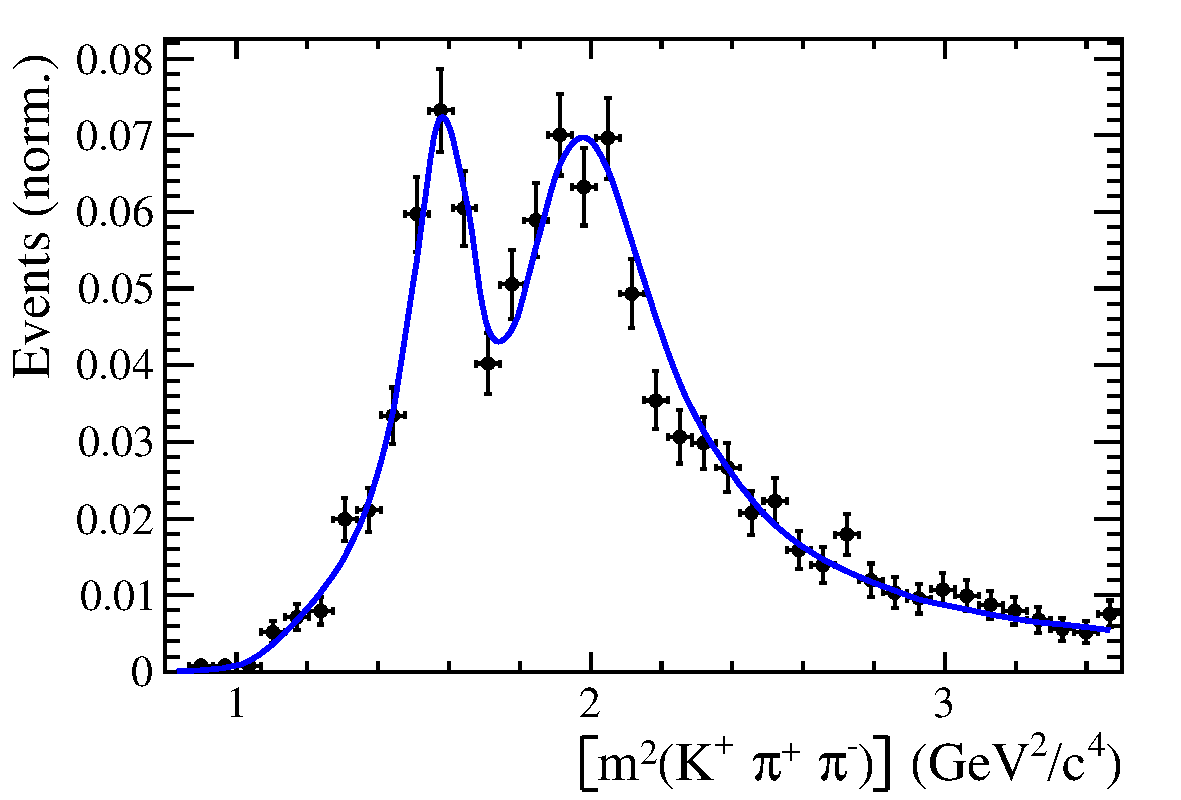
\includegraphics[width=0.45\textwidth, height = !]{figs/plots_toy/s_Kpipi-eps-converted-to.pdf}
		 
		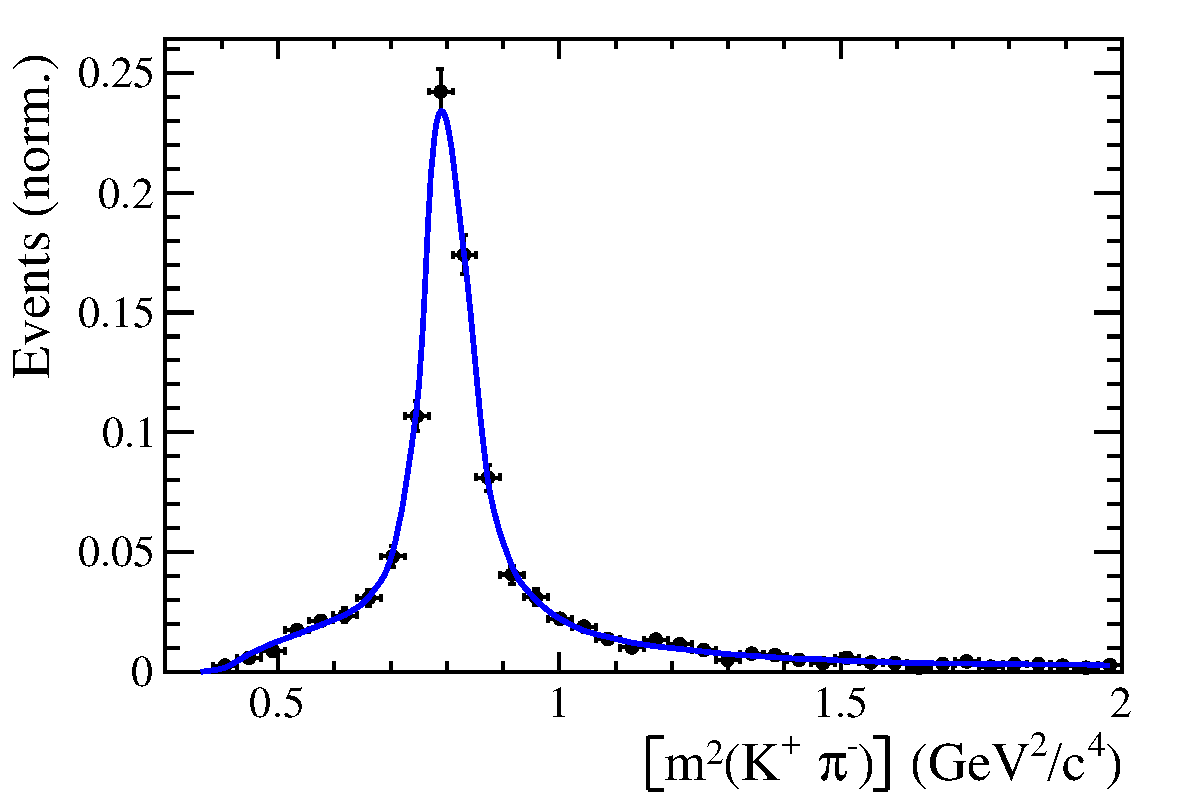
\includegraphics[width=0.45\textwidth, height = !]{figs/plots_toy/s_Kpi-eps-converted-to.pdf} 
		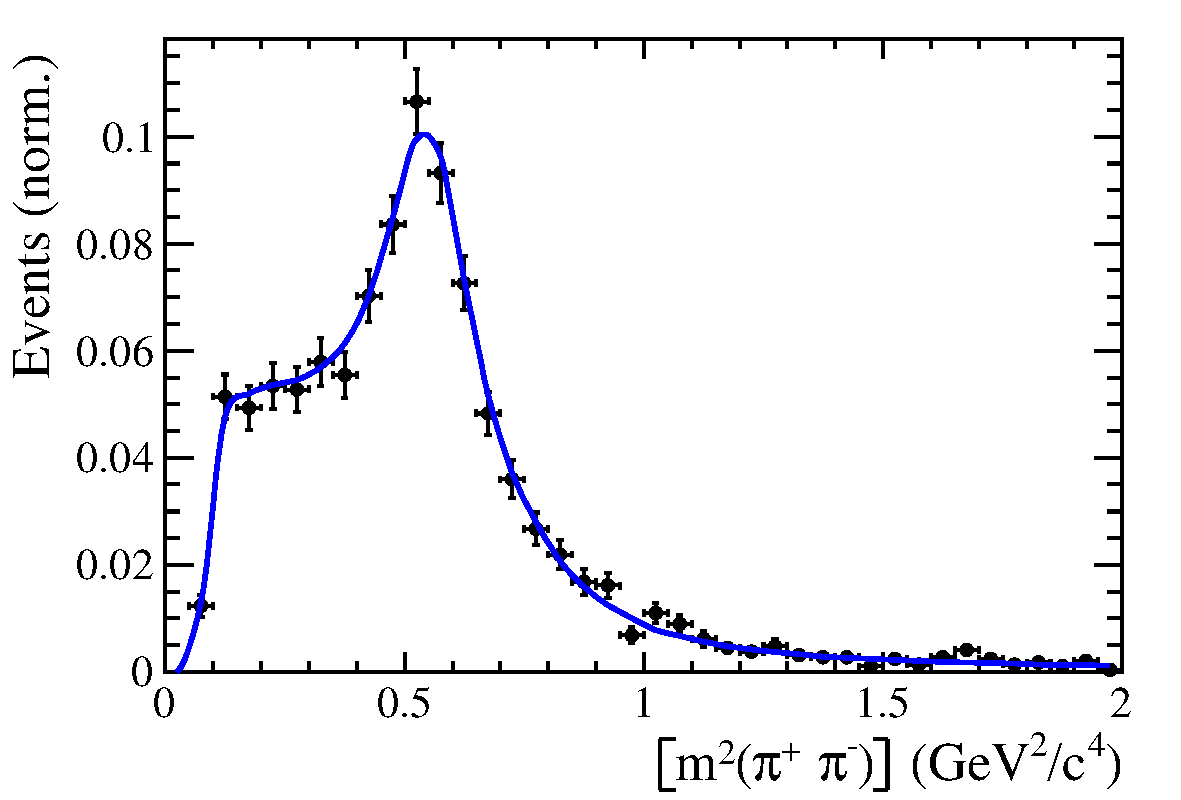
\includegraphics[width=0.45\textwidth, height = !]{figs/plots_toy/s_pipi-eps-converted-to.pdf}
		
		\caption{Example toy fit} 		
	\end{figure}				


	\begin{figure}[hp]
	\centering
		
%		$D_s^+ K^- \pi \pi$      \hspace{2cm}     $D_s^- K^+ \pi \pi$   \hspace{2cm}   Combined
%		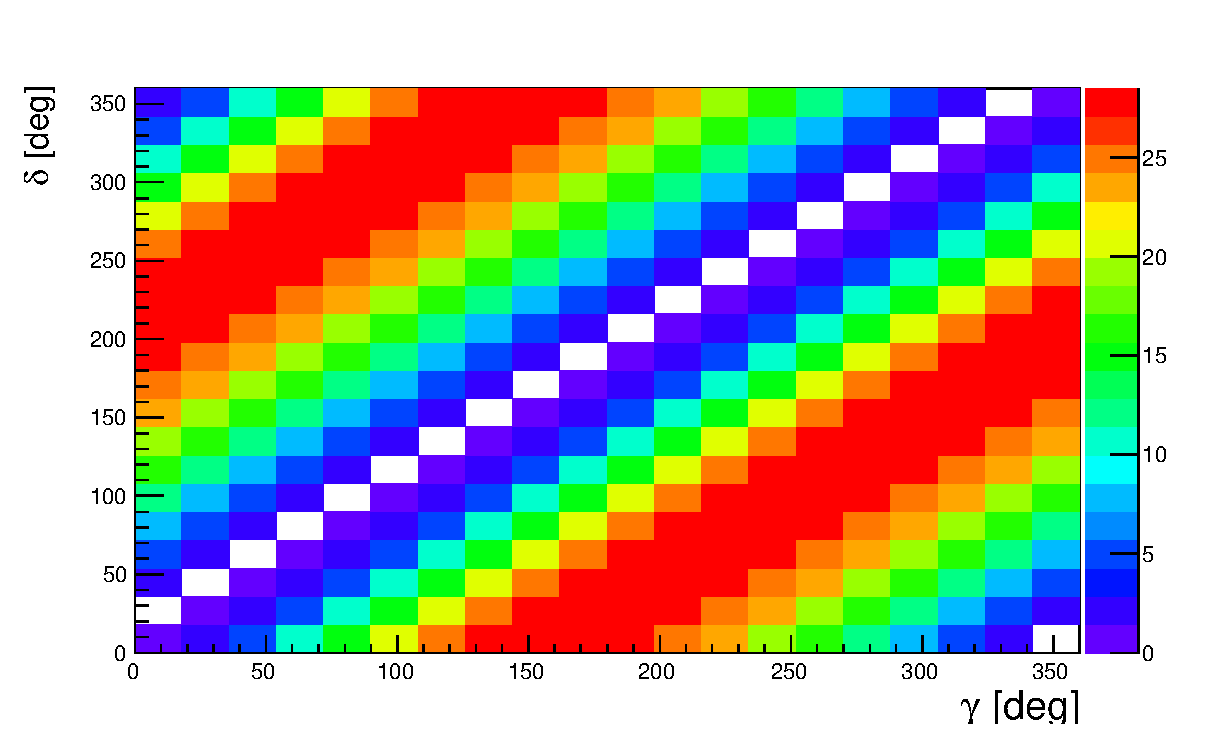
\includegraphics[width=0.4\textwidth, height = 4 cm{plots/LL_scan_m.eps} 
%		\includegraphics[width=0.4\textwidth, height = 4 cm]{plots/LL_scan_p.eps} 
		
		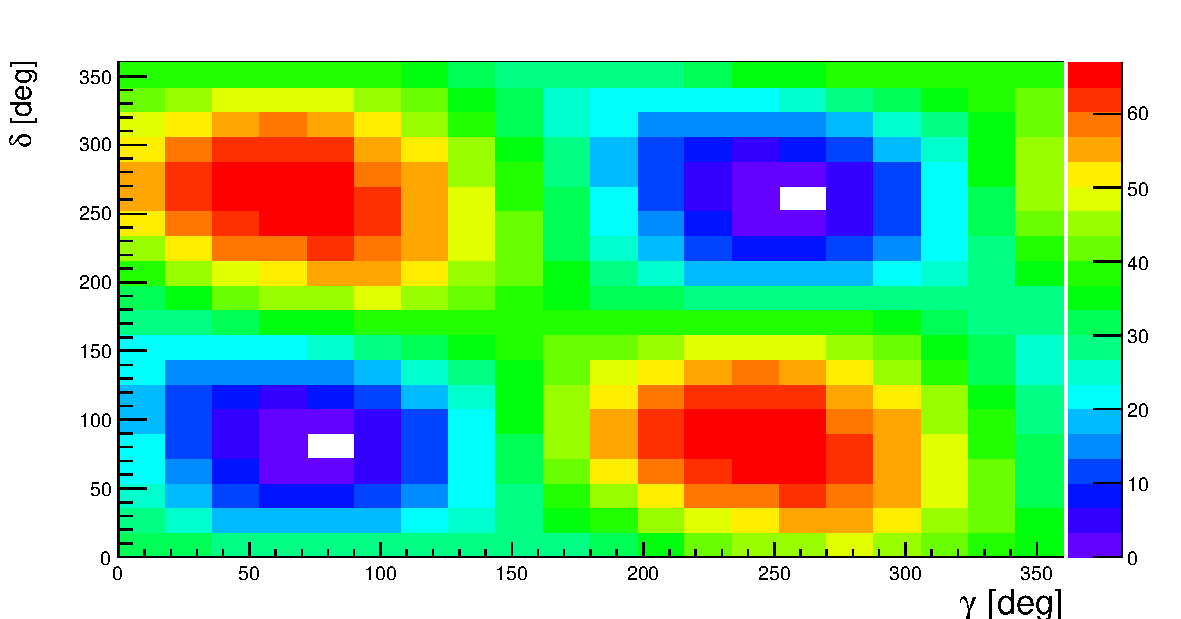
\includegraphics[width=0.45\textwidth, height = 4 cm]{plots/LL_scan-eps-converted-to.pdf} 
		
		Generated values: \\  $\gamma = 70^{\circ}, \delta = 100^{\circ}$ \\
		Fit result:    \\ $\gamma = 74 \pm 15^{\circ}, \delta = 84 \pm 15^{\circ}$ \\
		 ($\gamma = 254 \pm 15^{\circ}, \delta = 264 \pm 15^{\circ}$)

		\caption{Likelihood scan} 		

	\end{figure}	


	\begin{figure}[hp]
	\centering
		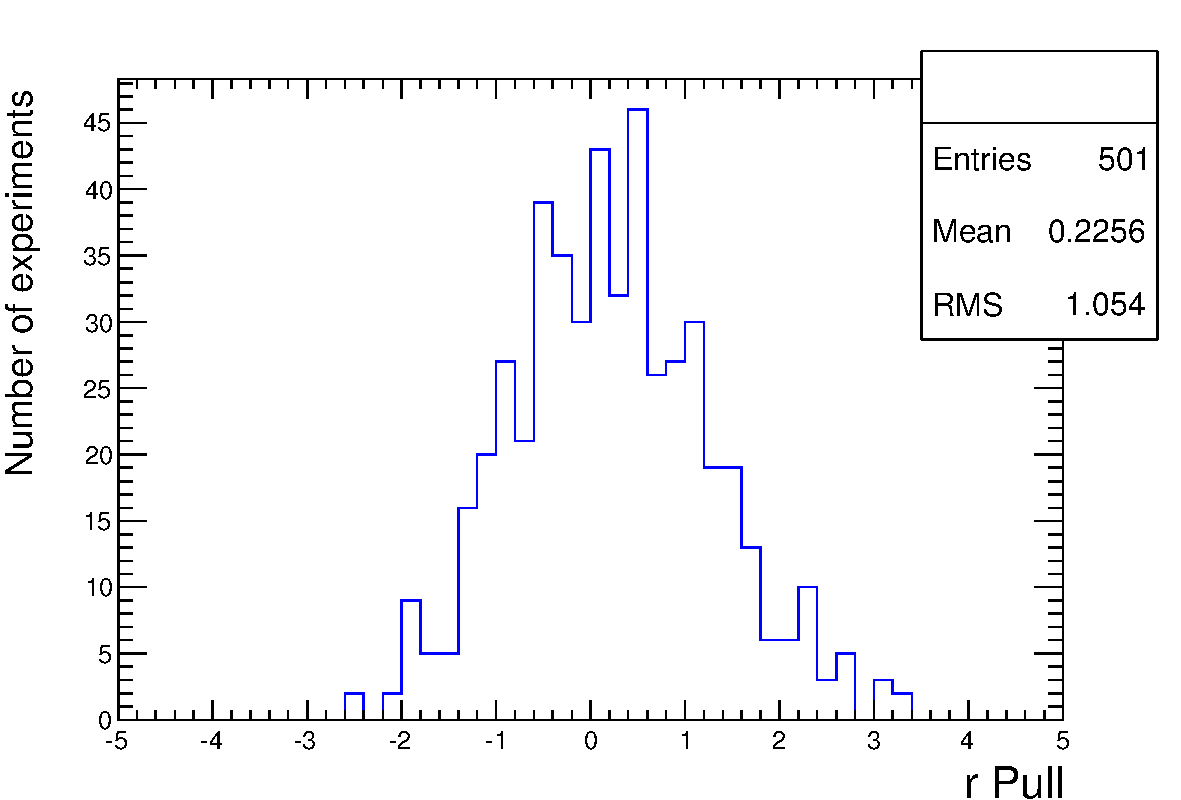
\includegraphics[width=0.4\textwidth, height = 3.cm]{figs/plots_toy/r_pull-eps-converted-to.pdf} 
		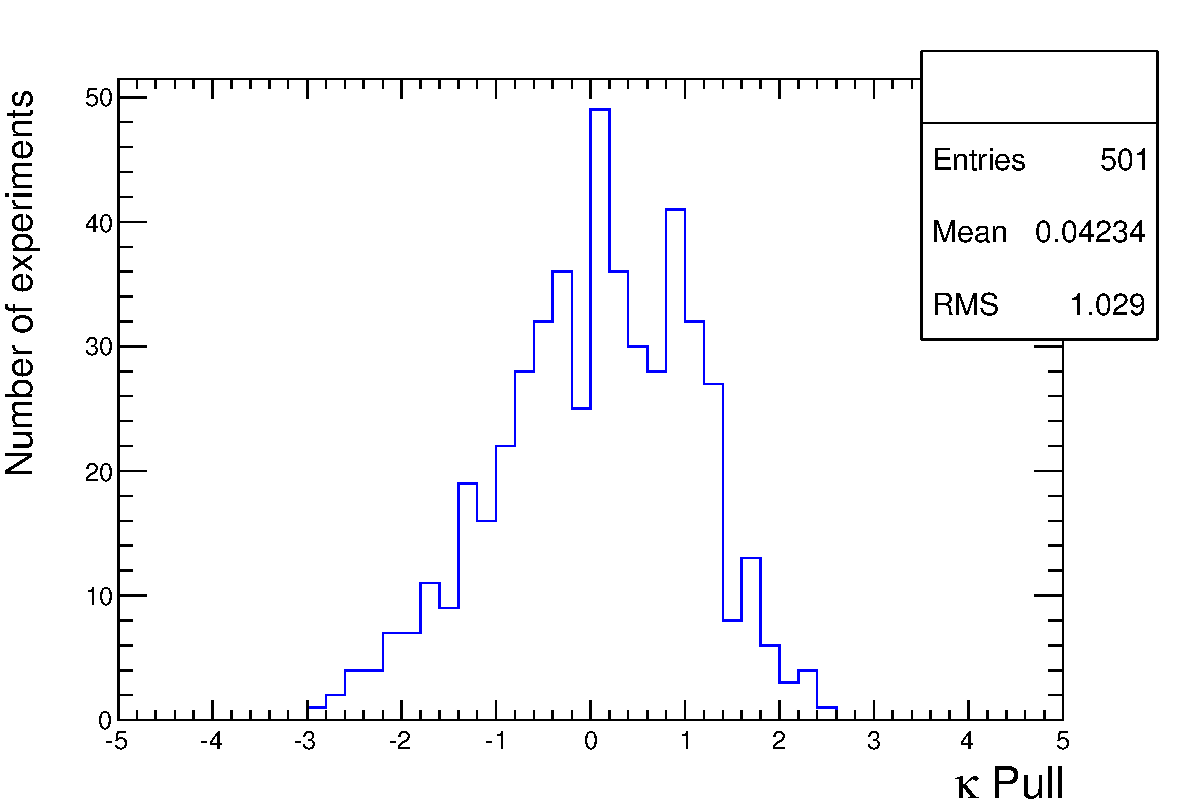
\includegraphics[width=0.4\textwidth, height = 3.cm]{figs/plots_toy/k_pull-eps-converted-to.pdf} 
		
		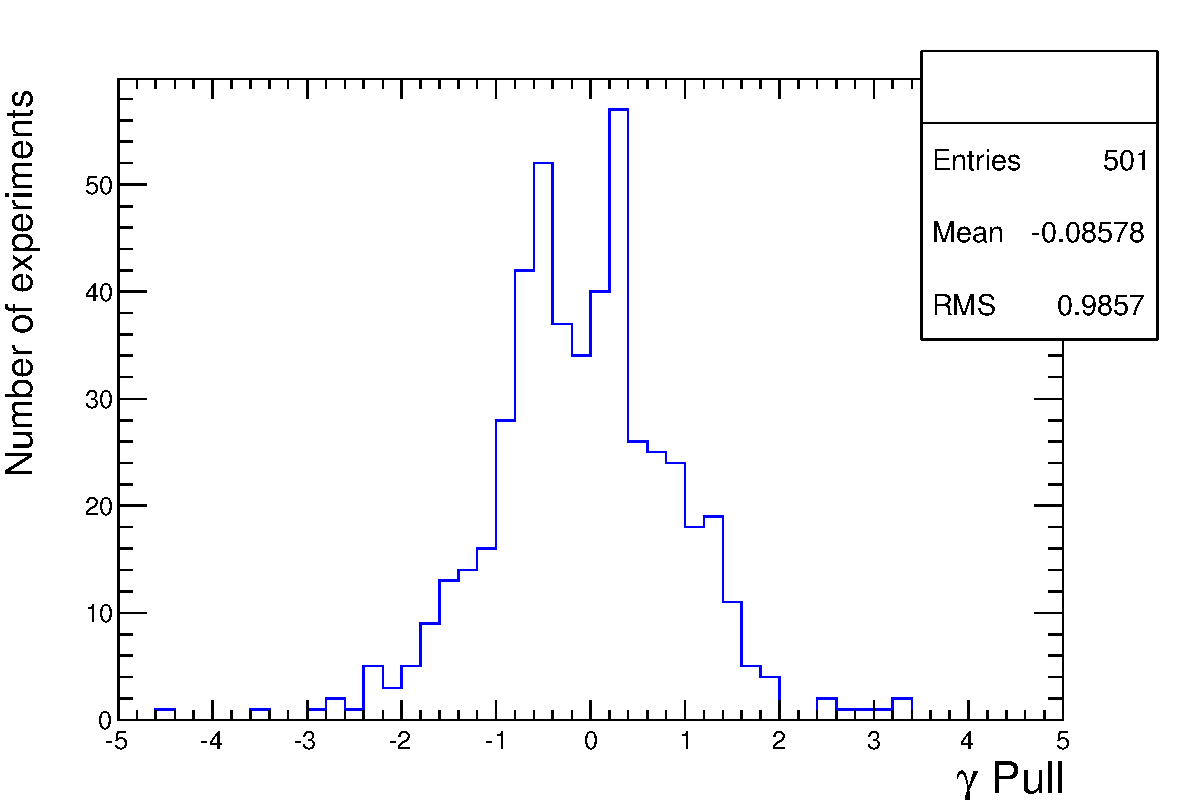
\includegraphics[width=0.4\textwidth, height = 3.cm]{figs/plots_toy/gamma_pull-eps-converted-to.pdf} 
		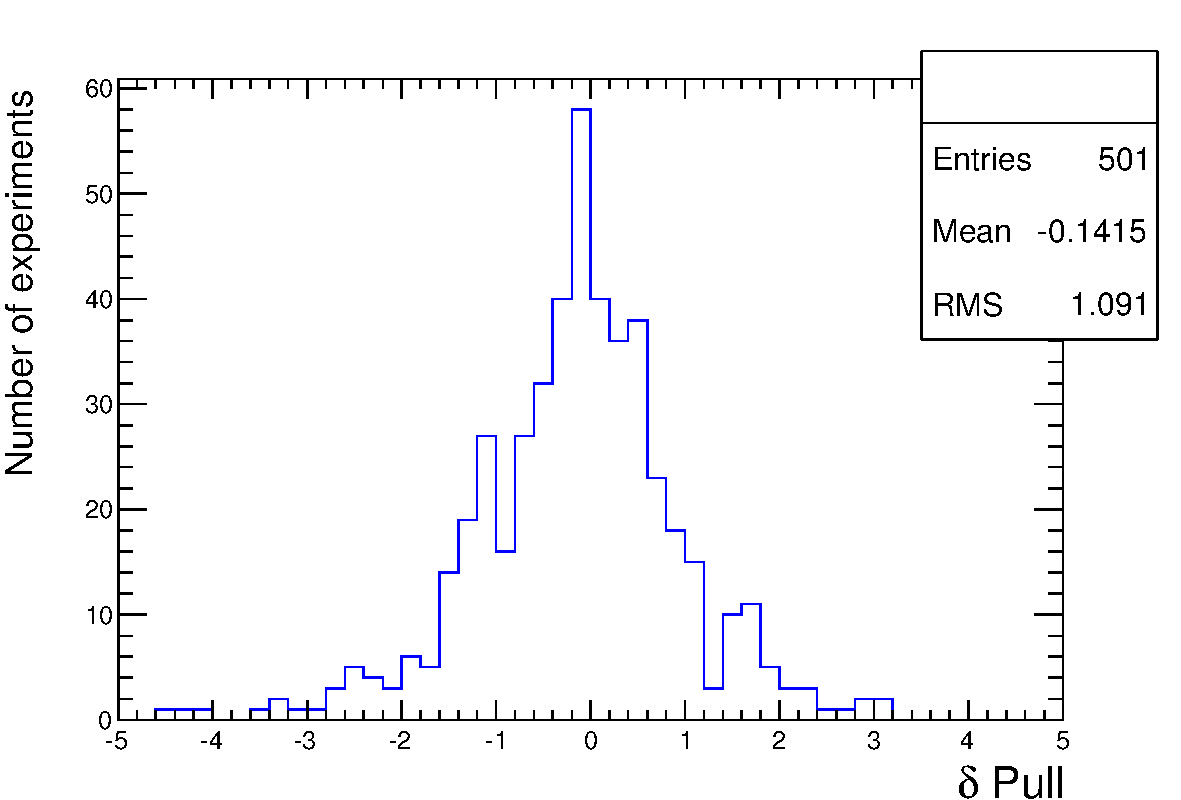
\includegraphics[width=0.4\textwidth, height = 3.cm]{figs/plots_toy/delta_pull-eps-converted-to.pdf} 

		\caption{Pulls} 		

	\end{figure}	
	

\clearpage	

\begin{table}[h]
	\caption{} 		
  \scriptsize
  \centering
  \begin{tabular}
    {l c c c c}
    \hline \hline
    & Generated &  Full PDF     &   Phasespace integrated  \\   \hline
	$r$ & 0.4 & $0.38 \pm 0.06$   &  unstable \\
	$\kappa$  & \textcolor{red}{0.2} & $0.23 \pm 0.13$ & 0.2 (fixed)  \\
	$\delta$ & 100 & $99 \pm 22$ &  unstable\\
	$\gamma$ & 70 & $70 \pm 17$  & unstable \\
    \hline \hline
  \end{tabular}

  \begin{tabular}
    {l c c c c}
    \hline \hline
    & Generated &  Full PDF    &   Phasespace integrated  \\   \hline
	$r$ & 0.4 & $0.44 \pm 0.07$      & $0.43 \pm 0.11$  \\
	$\kappa$  & \textcolor{red}{0.4} &$0.41 \pm 0.14$  & 0.4 (fixed)  \\
	$\delta$ & 100 & $101 \pm 19$  & $95 \pm 41$ \\
	$\gamma$ & 70 & $69 \pm 16$   & $66 \pm 40 $ \\
    \hline \hline
  \end{tabular}

  \begin{tabular}
    {l c c c c}
    \hline \hline
    & Generated &  Full PDF    &   Phasespace integrated  \\   \hline
	$r$ & 0.4 & $0.41 \pm 0.08$     & $0.39 \pm 0.11$  \\
	$\kappa$  & \textcolor{red}{0.6} & $0.60 \pm 0.13$  & 0.6 (fixed)  \\
	$\delta$ & 100 & $98 \pm 17$ & $92 \pm 25$ \\
	$\gamma$ & 70 & $68 \pm 17$ & $65 \pm 28$ \\
    \hline \hline
  \end{tabular}

  \begin{tabular}
    {l c c c c}
    \hline \hline
    & Generated &  Full PDF        &   Phasespace integrated  \\   \hline
	$r$ & 0.4 & $0.42 \pm 0.09$    &  $0.39 \pm 0.09$ \\
	$\kappa$  & \textcolor{red}{1.0} & $0.96 \pm 0.03$ &  1.0 (fixed)  \\
	$\delta$ & 100 & $100 \pm 17$ &  $100 \pm 17$  \\
	$\gamma$ & 70 & $66 \pm 17$ & $67 \pm 17$  \\
    \hline \hline
  \end{tabular}
\end{table}
